\documentclass[
  man,
  floatsintext,
  longtable,
  nolmodern,
  notxfonts,
  notimes,
  colorlinks=true,linkcolor=blue,citecolor=blue,urlcolor=blue]{apa7}

\usepackage{amsmath}
\usepackage{amssymb}




\RequirePackage{longtable}
\RequirePackage{threeparttablex}

\makeatletter
\renewcommand{\paragraph}{\@startsection{paragraph}{4}{\parindent}%
	{0\baselineskip \@plus 0.2ex \@minus 0.2ex}%
	{-.5em}%
	{\normalfont\normalsize\bfseries\typesectitle}}

\renewcommand{\subparagraph}[1]{\@startsection{subparagraph}{5}{0.5em}%
	{0\baselineskip \@plus 0.2ex \@minus 0.2ex}%
	{-\z@\relax}%
	{\normalfont\normalsize\bfseries\itshape\hspace{\parindent}{#1}\textit{\addperi}}{\relax}}
\makeatother




\usepackage{longtable, booktabs, multirow, multicol, colortbl, hhline, caption, array, float, xpatch}
\usepackage{subcaption}


\renewcommand\thesubfigure{\Alph{subfigure}}
\setcounter{topnumber}{2}
\setcounter{bottomnumber}{2}
\setcounter{totalnumber}{4}
\renewcommand{\topfraction}{0.85}
\renewcommand{\bottomfraction}{0.85}
\renewcommand{\textfraction}{0.15}
\renewcommand{\floatpagefraction}{0.7}

\usepackage{tcolorbox}
\tcbuselibrary{listings,theorems, breakable, skins}
\usepackage{fontawesome5}

\definecolor{quarto-callout-color}{HTML}{909090}
\definecolor{quarto-callout-note-color}{HTML}{0758E5}
\definecolor{quarto-callout-important-color}{HTML}{CC1914}
\definecolor{quarto-callout-warning-color}{HTML}{EB9113}
\definecolor{quarto-callout-tip-color}{HTML}{00A047}
\definecolor{quarto-callout-caution-color}{HTML}{FC5300}
\definecolor{quarto-callout-color-frame}{HTML}{ACACAC}
\definecolor{quarto-callout-note-color-frame}{HTML}{4582EC}
\definecolor{quarto-callout-important-color-frame}{HTML}{D9534F}
\definecolor{quarto-callout-warning-color-frame}{HTML}{F0AD4E}
\definecolor{quarto-callout-tip-color-frame}{HTML}{02B875}
\definecolor{quarto-callout-caution-color-frame}{HTML}{FD7E14}

%\newlength\Oldarrayrulewidth
%\newlength\Oldtabcolsep


\usepackage{hyperref}




\providecommand{\tightlist}{%
  \setlength{\itemsep}{0pt}\setlength{\parskip}{0pt}}
\usepackage{longtable,booktabs,array}
\usepackage{calc} % for calculating minipage widths
% Correct order of tables after \paragraph or \subparagraph
\usepackage{etoolbox}
\makeatletter
\patchcmd\longtable{\par}{\if@noskipsec\mbox{}\fi\par}{}{}
\makeatother
% Allow footnotes in longtable head/foot
\IfFileExists{footnotehyper.sty}{\usepackage{footnotehyper}}{\usepackage{footnote}}
\makesavenoteenv{longtable}

\usepackage{graphicx}
\makeatletter
\newsavebox\pandoc@box
\newcommand*\pandocbounded[1]{% scales image to fit in text height/width
  \sbox\pandoc@box{#1}%
  \Gscale@div\@tempa{\textheight}{\dimexpr\ht\pandoc@box+\dp\pandoc@box\relax}%
  \Gscale@div\@tempb{\linewidth}{\wd\pandoc@box}%
  \ifdim\@tempb\p@<\@tempa\p@\let\@tempa\@tempb\fi% select the smaller of both
  \ifdim\@tempa\p@<\p@\scalebox{\@tempa}{\usebox\pandoc@box}%
  \else\usebox{\pandoc@box}%
  \fi%
}
% Set default figure placement to htbp
\def\fps@figure{htbp}
\makeatother


% definitions for citeproc citations
\NewDocumentCommand\citeproctext{}{}
\NewDocumentCommand\citeproc{mm}{%
  \begingroup\def\citeproctext{#2}\cite{#1}\endgroup}
\makeatletter
 % allow citations to break across lines
 \let\@cite@ofmt\@firstofone
 % avoid brackets around text for \cite:
 \def\@biblabel#1{}
 \def\@cite#1#2{{#1\if@tempswa , #2\fi}}
\makeatother
\newlength{\cslhangindent}
\setlength{\cslhangindent}{1.5em}
\newlength{\csllabelwidth}
\setlength{\csllabelwidth}{3em}
\newenvironment{CSLReferences}[2] % #1 hanging-indent, #2 entry-spacing
 {\begin{list}{}{%
  \setlength{\itemindent}{0pt}
  \setlength{\leftmargin}{0pt}
  \setlength{\parsep}{0pt}
  % turn on hanging indent if param 1 is 1
  \ifodd #1
   \setlength{\leftmargin}{\cslhangindent}
   \setlength{\itemindent}{-1\cslhangindent}
  \fi
  % set entry spacing
  \setlength{\itemsep}{#2\baselineskip}}}
 {\end{list}}
\usepackage{calc}
\newcommand{\CSLBlock}[1]{\hfill\break\parbox[t]{\linewidth}{\strut\ignorespaces#1\strut}}
\newcommand{\CSLLeftMargin}[1]{\parbox[t]{\csllabelwidth}{\strut#1\strut}}
\newcommand{\CSLRightInline}[1]{\parbox[t]{\linewidth - \csllabelwidth}{\strut#1\strut}}
\newcommand{\CSLIndent}[1]{\hspace{\cslhangindent}#1}





\usepackage{newtx}

\defaultfontfeatures{Scale=MatchLowercase}
\defaultfontfeatures[\rmfamily]{Ligatures=TeX,Scale=1}





\title{The Link Function Problem in Psychological Interaction Testing}


\shorttitle{Link Functions and Interactions}


\usepackage{etoolbox}









\authorsnames[{1},{2},{1},{1},{1}]{Margherita Calderan,Filippo
Gambarota,Laura Sità,Tommaso Feraco,Enrico Toffalini}







\authorsaffiliations{
{Department of General Psychology, University of Padova},{Department of
Developmental Psychology and Socialization, University of Padova}}




\leftheader{Calderan, Gambarota, Sità, Feraco and Toffalini}



\abstract{Equal differences on one scale become different differences on
another scale. This is crucial for interaction testing because an
interaction is a difference between differences, and in psychological
research the observed response and the construct of interest are often
expressed on different scales. Therefore, the same data can show an
interaction on one scale and not on another. Generalized Linear Models
make this problem explicit by separating two decisions: the family,
which describes the nature of the response variable, and the link
function, which sets the scale on which effects are additive. Because a
model without an interaction term is additive on the link scale,
choosing a link is choosing what `no interaction' means. The paper has
two connected parts. First, a preregistered review of recent articles
from five prominent psychology journals shows that interaction testing
is routinely performed in research, that the link function is most often
unspecified, and that constrained outcomes are frequently analyzed with
gaussian identity-link models. Second, worked examples and simulations
develop three common response formats: forced-choice accuracy with a
chance floor, within-family link choices (logit vs probit), and sum
scores as a measurement case, and quantify how a plausible-looking link
can turn an additive structure on one scale into a statistically
significant interaction on another. A final diagnostic simulation shows
that residual checks, a link test, and AIC comparisons give uneven
protection and do not by themselves decide which scale the scientific
claim concerns. Interaction claims remain underspecified until
researchers state, justify, and probe the scale on which no interaction
is assumed. }

\keywords{interactions, moderation, generalized linear models, link
functions, model misspecification}

\authornote{\par{\addORCIDlink{Margherita
Calderan}{0009-0005-5668-5162}}\par{\addORCIDlink{Filippo
Gambarota}{0000-0002-6666-1747}}\par{\addORCIDlink{Laura
Sità}{0009-0000-6017-9979}}\par{\addORCIDlink{Tommaso
Feraco}{0000-0002-8920-5330}}\par{\addORCIDlink{Enrico
Toffalini}{0000-0002-1404-5133}} 
\par{ }
\par{       }
\par{Correspondence concerning this article should be addressed
to Enrico Toffalini, Department of General Psychology, University of
Padova, Via Venezia
8, Padova 35131, Italy, Email: \href{mailto:enrico.toffalini@unipd.it}{enrico.toffalini@unipd.it}}
}

\makeatletter
\let\endoldlt\endlongtable
\def\endlongtable{
\hline
\endoldlt
}
\makeatother

\urlstyle{same}



% Single-space table bodies so tables fit in text (floatsintext).
% Wrapped lines inside a cell are set slightly tighter than normal and
% each row gets a little extra vertical air, so a line break inside a
% cell is not mistaken for the start of a new table row.
\usepackage{etoolbox}
\usepackage{array}
\AtBeginEnvironment{longtable}{%
  \linespread{0.95}\selectfont
  \setlength{\extrarowheight}{6pt}}
\AtBeginEnvironment{tabular}{%
  \linespread{0.95}\selectfont
  \setlength{\extrarowheight}{6pt}}
\usepackage{float}
\raggedbottom
\makeatletter
\@ifpackageloaded{tcolorbox}{}{\usepackage[skins,breakable]{tcolorbox}}
\@ifpackageloaded{fontawesome5}{}{\usepackage{fontawesome5}}
\definecolor{quarto-callout-color}{HTML}{909090}
\definecolor{quarto-callout-note-color}{HTML}{0758E5}
\definecolor{quarto-callout-important-color}{HTML}{CC1914}
\definecolor{quarto-callout-warning-color}{HTML}{EB9113}
\definecolor{quarto-callout-tip-color}{HTML}{00A047}
\definecolor{quarto-callout-caution-color}{HTML}{FC5300}
\definecolor{quarto-callout-color-frame}{HTML}{acacac}
\definecolor{quarto-callout-note-color-frame}{HTML}{4582ec}
\definecolor{quarto-callout-important-color-frame}{HTML}{d9534f}
\definecolor{quarto-callout-warning-color-frame}{HTML}{f0ad4e}
\definecolor{quarto-callout-tip-color-frame}{HTML}{02b875}
\definecolor{quarto-callout-caution-color-frame}{HTML}{fd7e14}
\makeatother
\makeatletter
\@ifpackageloaded{caption}{}{\usepackage{caption}}
\AtBeginDocument{%
\ifdefined\contentsname
  \renewcommand*\contentsname{Table of contents}
\else
  \newcommand\contentsname{Table of contents}
\fi
\ifdefined\listfigurename
  \renewcommand*\listfigurename{List of Figures}
\else
  \newcommand\listfigurename{List of Figures}
\fi
\ifdefined\listtablename
  \renewcommand*\listtablename{List of Tables}
\else
  \newcommand\listtablename{List of Tables}
\fi
\ifdefined\figurename
  \renewcommand*\figurename{Figure}
\else
  \newcommand\figurename{Figure}
\fi
\ifdefined\tablename
  \renewcommand*\tablename{Table}
\else
  \newcommand\tablename{Table}
\fi
}
\@ifpackageloaded{float}{}{\usepackage{float}}
\floatstyle{ruled}
\@ifundefined{c@chapter}{\newfloat{codelisting}{h}{lop}}{\newfloat{codelisting}{h}{lop}[chapter]}
\floatname{codelisting}{Listing}
\newcommand*\listoflistings{\listof{codelisting}{List of Listings}}
\makeatother
\makeatletter
\makeatother
\makeatletter
\@ifpackageloaded{caption}{}{\usepackage{caption}}
\@ifpackageloaded{subcaption}{}{\usepackage{subcaption}}
\makeatother

% From https://tex.stackexchange.com/a/645996/211326
%%% apa7 doesn't want to add appendix section titles in the toc
%%% let's make it do it
\makeatletter
\xpatchcmd{\appendix}
  {\par}
  {\addcontentsline{toc}{section}{\@currentlabelname}\par}
  {}{}
\makeatother

%% Disable longtable counter
%% https://tex.stackexchange.com/a/248395/211326

\usepackage{etoolbox}

\makeatletter
\patchcmd{\LT@caption}
  {\bgroup}
  {\bgroup\global\LTpatch@captiontrue}
  {}{}
\patchcmd{\longtable}
  {\par}
  {\par\global\LTpatch@captionfalse}
  {}{}
\apptocmd{\endlongtable}
  {\ifLTpatch@caption\else\addtocounter{table}{-1}\fi}
  {}{}
\newif\ifLTpatch@caption
\makeatother

\begin{document}

\maketitle




\setlength\LTleft{0pt}




\subsection{}\label{section}

We start with a very simplified example. Two populations of children
(e.g., clinical vs neurotypical) differ in their overall error rates on
a task, and errors decrease with age in both.
Figure~\ref{fig-simple-count-example} samples simulated data from such a
scenario. In the left panel (observed response), errors decline with age
in both groups, and the difference between groups is much larger at age
six than at age ten. Is there an age-by-group interaction here?

\begin{figure}[h]

\caption{\label{fig-simple-count-example}Simulated error counts for two
groups of children aged 6 to 10, shown on the observed count scale
(left) and on the log scale (right). The two groups have exactly the
same age effect on the log of the expected error count, so on the log
scale the two fitted lines are parallel, with a constant group gap at
every age. Mapped back onto the count scale, the same model produces
converging curves, so the group difference shrinks with age. Whether
this pattern is an interaction depends on the scale on which effects are
assumed to add: on the count scale the group difference changes with
age; on the log scale it does not.}

\centering{

\pandocbounded{
\includegraphics[keepaspectratio]{paper-v2_files/figure-pdf/fig-simple-count-example-1.pdf}}

}

\end{figure}%

Because an interaction is a difference between differences, the question
is whether the group difference itself changes with age. On the observed
count scale, the group effect does appear to shrink as age increases, so
it looks like an interaction. But looking at the same data on the
log-scale (Figure~\ref{fig-simple-count-example}, right panel), both
groups have the same age slope, meaning their fitted lines are parallel.
A constant difference on the log scale corresponds to a constant ratio
on the count scale, so the absolute gap between groups is proportional
to the baseline and shrinks as errors decline with age. Whether we call
this an interaction is not a fact about the data, it depends on which
scale we assume effects add up linearly on. Additive on the log scale
means multiplicative (and non-parallel) on the count scale, and vice
versa.

This ambiguity extends far beyond this single illustration, as
interaction hypotheses are widespread in psychological research and
often represent the central target of inquiry
(\citeproc{ref-domingue2024}{Domingue et al., 2024};
\citeproc{ref-mccabe2022}{McCabe et al., 2022};
\citeproc{ref-rohrer2021}{Rohrer \& Arslan, 2021}). Whenever researchers
ask whether an effect is moderated, or whether it holds only under
certain conditions, they are asserting that the impact of one variable
depends on another. This count example therefore demonstrates that the
reality of such a claim can shift entirely based on the scale on which
those differences are computed.

In psychology, this scale dependence has a characteristic source in
measurement. Researchers routinely conceptualize constructs such as
cognitive ability or symptom severity as continuous latent dimensions
(\citeproc{ref-embretsonReise2000}{Embretson \& Reise, 2000};
\citeproc{ref-wagenmakers2012}{Wagenmakers et al., 2012}). Those
dimensions are rarely observed directly; what reaches the data are
bounded, discrete quantities, such as counts, ratings, and accuracy
scores that carry floors, ceilings, and chance levels. Each measurement
scale imposes its own mapping from the latent dimension to the observed
response. Where the mapping compresses, a constant effect on the latent
dimension appears as a shrinking effect on the observed response: a
group or condition closer to a bound has less room to move, and can look
less affected by a manipulation, than a group or condition farther away
from bounds (e.g., Figure~\ref{fig-simple-count-example}, left panel).

Generalized linear models (GLMs) make this mapping explicit and give it
a standard vocabulary (\citeproc{ref-mccullaghnelder1989}{McCullagh \&
Nelder, 1989}; \citeproc{ref-nelderwedderburn1972}{Nelder \& Wedderburn,
1972}), separating two choices that are easy to conflate, (1) the
outcome family, which describes the response, and (2) the link function,
which sets the scale on which effects combine (Box 1).

\begin{tcolorbox}[enhanced jigsaw, titlerule=0mm, colbacktitle=quarto-callout-note-color!10!white, colback=white, arc=.35mm, title={Box 1: Generalized linear models: outcome family and link function}, toptitle=1mm, left=2mm, toprule=.15mm, coltitle=black, colframe=quarto-callout-note-color-frame, opacityback=0, opacitybacktitle=0.6, breakable, leftrule=.75mm, bottomtitle=1mm, rightrule=.15mm, bottomrule=.15mm]

The \emph{outcome family} is the distribution assumed for the response.
It defines which values the outcome can take and how observations vary
around their expectation. The \emph{link function}, \(g(\cdot)\), maps
the expected outcome, \(\mu_i = E(Y_i)\), onto the linear predictor,
\(\eta_i\), the scale on which the model is additive. With two
predictors and their interaction term,
\[g(\mu_i) = \eta_i, \qquad \eta_i = \beta_0 + \beta_1 X_i + \beta_2 Z_i + \beta_3 X_i Z_i.\]

The inverse link, \(g^{-1}(\cdot)\), maps this additive structure back
onto the expected response. Its familiar role is to keep expected values
within the admissible range of a constrained outcome: \(\exp(\eta)\)
keeps expected counts positive, and the inverse logit keeps
probabilities between 0 and 1. Less obviously, this also fixes what the
absence of an interaction, \(\beta_3 = 0\), means in the fitted model.
The product-term coefficient \(\beta_3\) is therefore an interaction on
the link scale. A response-scale interaction is a different quantity: a
difference between expected differences on the observed outcome, for
example, whether the group difference in expected errors changes with
age in Figure~\ref{fig-simple-count-example}. Unless the link is the
identity, the two quantities can disagree
(\citeproc{ref-ainorton2003}{Ai \& Norton, 2003};
\citeproc{ref-mccabe2022}{McCabe et al., 2022};
\citeproc{ref-mize2019}{Mize, 2019}). Each family has a canonical link,
which is the one that arises directly from the family's mathematical
form, but it is a convenient default and other links are legitimate. A
Gaussian linear model is the special case that combines a Gaussian
family with an identity link, so the additive scale and the response
scale coincide and the scale question is invisible. The model behind
Figure~\ref{fig-simple-count-example} is a Poisson family with a log
link. The family respects that errors are non-negative counts, and the
link places additivity on the log scale.

\end{tcolorbox}

Often the outcome family is chosen with care while the link function is
left at its software default, fixing the scale of additivity without
deliberation. Two models can share a family and still place additivity
on different scales. For example, a Gamma family suits reaction times
data; within that family, a log link makes effects additive in log
milliseconds, a proportional change, and the canonical inverse link
makes them additive in reciprocal means, a change in speed. A binomial
family fits correct-versus-incorrect responses and leaves the link open
among logit, probit, chance-corrected, and other forms.

The scale dependence of interactions has long been recognized. Loftus
showed that interactions involving response probabilities are meaningful
only relative to a mapping between observed and theoretical scales
(\citeproc{ref-loftus1978}{Loftus, 1978}), and Cox formalized
interaction as a model-relative concept tied to transformation and
interpretation (\citeproc{ref-cox1984}{Cox, 1984}). Busemeyer and Jones
carried the same point into the measurement model, where the conclusion
about how two variables combine depends on the model assumed to link
responses to the quantities they measure
(\citeproc{ref-busemeyer1983}{Busemeyer \& Jones, 1983}). Lubinski and
Humphreys showed that the specification choices alone can produce the
appearance of an interaction where the generating process contains none
(\citeproc{ref-lubinski1990}{Lubinski \& Humphreys, 1990}).

More recently, Wagenmakers and colleagues separated removable from
nonremovable interactions (\citeproc{ref-wagenmakers2012}{Wagenmakers et
al., 2012}). A removable interaction can be undone by a monotonic
transformation of the dependent variable, which makes it a property of
the measurement scale, whereas a nonremovable one (typically a
cross-over) persists under any such transformation. Rohrer and Arslan
showed that the same interaction can be positive, null, or negative
depending on the scale chosen for the outcome, so the appropriate test
follows from the scale on which the hypothesis is posed
(\citeproc{ref-rohrer2021}{Rohrer \& Arslan, 2021}). Rimpler and
colleagues added that a product term assumes one predictor's effect
changes at a constant rate across levels of the other, and so
misrepresents any dependence that does not take that form, such as a
threshold effect (\citeproc{ref-rimpler2026}{Rimpler et al., 2026}). In
GLMs specifically, the product-term coefficient refers to the link scale
and does not equal the interaction on the response scale, so a question
about the response scale should be answered with marginal effects
(\citeproc{ref-ainorton2003}{Ai \& Norton, 2003};
\citeproc{ref-mccabe2022}{McCabe et al., 2022};
\citeproc{ref-mize2019}{Mize, 2019}; \citeproc{ref-rohrer2026}{Rohrer \&
Arel-Bundock, 2026}).

Domingue and colleagues demonstrated that outcome-model misspecification
can produce false interaction findings for binary, count, and censored
outcomes (\citeproc{ref-domingue2024}{Domingue et al., 2024}), and
Liddell and Kruschke showed that treating ordinal responses as metric
can inflate error rates for interactions
(\citeproc{ref-liddellkruschke2018}{Liddell \& Kruschke, 2018}). Czado
and Santner, and later Yu and Huang, studied the inferential
consequences of link misspecification in binary GLMs and GLMMs
(\citeproc{ref-czadosantner1992}{Czado \& Santner, 1992};
\citeproc{ref-yuhuang2019}{Yu \& Huang, 2019}). Beyond the scale
question, interaction estimates are fragile for other reasons, including
small effects, low reliability, and limited power
(\citeproc{ref-baranger2023}{Baranger et al., 2023};
\citeproc{ref-castillo2026}{Castillo et al., 2026}).

This literature spans nearly five decades, but whether applied practice
has absorbed the warning is still unaddressed. The present article
approaches that gap from two directions. We first document current
practice with a preregistered review of recent empirical articles in
five prominent psychology journals, quantifying how often interactions
are tested, how often the outcome family and link function are made
explicit, and which response formats predominate. We then develop a
framework that separates outcome family, link function, and target
metric, and work it through three common response formats, namely
forced-choice accuracy with a chance floor, sum scores, and
within-family link choices such as logit versus probit, using
simulations to quantify how often an inadequate link turns a purely
additive structure into a statistically significant interaction and
whether standard diagnostics detect the misspecification.

These simulations take up the case in which the outcome family is
already broadly plausible and the link alone sets a disputable
no-interaction baseline, the common situation for bounded and
chance-limited psychological outcomes. Work on misspecification has
largely varied the outcome model as a whole
(\citeproc{ref-domingue2024}{Domingue et al., 2024};
\citeproc{ref-liddellkruschke2018}{Liddell \& Kruschke, 2018}), whereas
here the family stays fixed and the link carries the entire disagreement
about what counts as no interaction. An interaction that appears on a
scale other than the generating one is then a genuine mathematical
property of that scale (\citeproc{ref-cox1984}{Cox, 1984};
\citeproc{ref-domingue2024}{Domingue et al., 2024};
\citeproc{ref-loftus1978}{Loftus, 1978};
\citeproc{ref-mccabe2022}{McCabe et al., 2022}), correct where it was
computed and troublesome only when the claim is carried to a different
scale. Because the generating scale is known in a simulation, we can
call such a result a pseudo-interaction, an interaction that is zero on
the generating scale and nonzero on another fitted scale because the two
encode different additivity baselines. In empirical data, where the
generating scale is unknown, we describe interaction conclusions as
link-sensitive, conditional on the fitted scale, or unstable across
plausible links. Table~\ref{tbl-link-aware-workflow} summarizes these
insights into a practical workflow for applied research.

Technical details are reported in Supplement A; a broader precomputed
sensitivity atlas varying sample size, main-effect magnitude, the
intercept, and selected design parameters is reported in Supplement B.

\section{Current Practice in Psychological Interaction Testing: A
Preregistered
Review}\label{current-practice-in-psychological-interaction-testing-a-preregistered-review}

The review asks how often psychological articles test interactions, and
how often they make the outcome family and link function explicit enough
for a reader to know which interaction claim was tested. To our
knowledge, it is the first review to quantify link-function reporting in
psychological interaction tests. The coding is descriptive, so it
documents reporting practice rather than the correctness of any
substantive conclusion.

\subsection{Review Method}\label{review-method}

The protocol was preregistered before any record was screened
(\url{https://osf.io/bdu73/}), together with the coding data dictionary.
The essentials are given here; the full protocol, sampling frame, and
reliability are in Supplement A.

Following the preregistration, we sampled one journal from each of five
areas: \emph{Psychological Science} (general), \emph{Journal of
Experimental Psychology: General} (experimental), \emph{Journal of
Personality and Social Psychology} (social), \emph{Developmental
Science} (developmental), and \emph{Psychological Medicine} (clinical).
The five were selected on preregistered discretionary criteria: a
first-quartile 2023 Impact Factor, a broad rather than narrowly
specialized scope, not primarily publishing reviews, and strong
reputation in their field, as jointly judged by the coauthors. From each
journal's full set of 2024 articles in Scopus, records were screened in
a fixed random order until 40 eligible interaction-testing articles were
reached, for a preregistered total of 200. Because screening stopped
once 40 interaction-testing articles were reached, the number of records
screened, and therefore the denominator of the eligibility proportion,
varied across journals. Eligible articles were empirical reports of
original research; reviews, meta-analyses, editorials, theoretical and
qualitative-only articles, replication-only studies, and psychometric
validation studies were excluded. Detailed coding was applied only to
articles testing at least one interaction, and only to observed-outcome
analyses: articles whose relevant tests were purely latent-variable or
structural-equation models fell outside the coding scheme (12 such
exclusions).

Each interaction-testing article was independently coded by two
researchers, with disagreements resolved by discussion or by consulting
the other coauthors. Generative AI tools were used only as an optional
aid to locate passages within an article; all coding used in the review
is human.

For each article, the coders recorded five things: whether at least one
tested interaction used a non-identity link; whether the link function
was explicitly reported; whether at least one interaction applied an
incorrect identity-link analysis; whether at least one such interaction
was statistically significant, or interpreted analogously in a Bayesian
analysis; and which response-variable types were analyzed.

By a formally incorrect identity-link analysis we mean a Gaussian linear
regression with an identity link applied to an outcome with formal
constraints, such as bounds, discreteness, positivity, or a known chance
level. This is a conservative screening flag, applied only when the
constraint was identifiable from the report and does not imply the
substantive conclusion is wrong. The label is defined relative to the
constrained process that generates the outcome (if the observed score
were explicitly justified as the target metric, identity-link additivity
would instead be a defensible modeling choice, a distinction we develop
in the following sections).

The full operational rules the coders followed, including borderline
cases, are tabulated in Supplement A. Interrater agreement on the
double-coded records was high (Cohen's \(\kappa\) between 0.66 and
0.81); per-variable agreement and coder margins are reported in
Supplement A. Preregistered variable definitions, operational coding
rules, variable-specific agreement, and by-journal results are also
reported in Supplement A, Section S2.

\subsection{Review Findings}\label{review-findings}

First, interaction testing was common. Screening yielded 331 eligible
empirical articles, of which 200 tested at least one interaction,
60.4\%. Under the stopping rule this proportion describes the records
screened rather than a fixed-denominator sample, so we report it
descriptively and treat the per-journal proportions as the more
informative summary: these ranged from 38.1\% in Psychological Medicine
to 85.1\% in Journal of Experimental Psychology: General.

Second, model-scale reporting was uncommon. Among the 200
interaction-testing articles, 58 used at least one non-identity link
function, 29\%, 95\% CI {[}23.2, 35.6{]}, and only 46 explicitly
reported the link function, 23\%, 95\% CI {[}17.7, 29.3{]}. Thus, in
about 77.0\% of interaction-testing articles, the link function was not
explicitly stated.

Even the 46 explicit cases rest on a rule looser than the preregistered
one, which required a declaration of the link and treated naming a
family or a generalized linear model as insufficient. In coding we also
accepted link-specific model names, because in practice they identify
the link: ``logistic regression'' names the logit and ``probit
regression'' the probit. We also accepted ``Poisson regression'', which
names a family whose standard link is the log. The stricter
preregistered rule would give a lower count.

Third, constrained outcomes were often analyzed on the identity scale.
Among the 200 interaction-testing articles, 144 included at least one
formally incorrect identity-link analysis of a constrained observed
outcome, 72\%, 95\% CI {[}65.4, 77.8{]}. As noted, this is a
conservative screening count, flagged only when the constraint was clear
from the report. Of these 144 cases, 124 reported at least one
statistically significant interaction, 86.1\%, 95\% CI {[}79.5, 90.8{]}.
This is not a comparison, because significance was coded only within the
flagged analyses; that is, 62.0\% of all interaction-testing articles
combined a constrained outcome, an identity-link analysis, and a
significant interaction claim. This is the same concern raised by work
on outcome-model mismatch in interaction testing
(\citeproc{ref-domingue2024}{Domingue et al., 2024};
\citeproc{ref-liddellkruschke2018}{Liddell \& Kruschke, 2018}).
Table~\ref{tbl-current-practice} summarizes these results.

\begin{table}

{\caption{{Descriptive summary of the preregistered review. Formally
incorrect identity-link analyses of constrained observed outcomes are
cases where the reported outcome had formal constraints that make
identity-link additivity formally incorrect as a generative model unless
explicitly justified as an approximation or as the target observed-score
metric. The interval on the eligibility row is reported for completeness
only: screening stopped at 40 interaction-testing articles per journal,
denominator was not fixed by design.}{\label{tbl-current-practice}}}
\vspace{-20pt}}

\begin{longtable}[]{@{}
  >{\raggedright\arraybackslash}p{(\linewidth - 8\tabcolsep) * \real{0.7622}}
  >{\raggedleft\arraybackslash}p{(\linewidth - 8\tabcolsep) * \real{0.0280}}
  >{\raggedleft\arraybackslash}p{(\linewidth - 8\tabcolsep) * \real{0.0490}}
  >{\raggedleft\arraybackslash}p{(\linewidth - 8\tabcolsep) * \real{0.0490}}
  >{\raggedleft\arraybackslash}p{(\linewidth - 8\tabcolsep) * \real{0.1119}}@{}}
\toprule\noalign{}
\begin{minipage}[b]{\linewidth}\raggedright
Quantity
\end{minipage} & \begin{minipage}[b]{\linewidth}\raggedleft
n
\end{minipage} & \begin{minipage}[b]{\linewidth}\raggedleft
Denom.
\end{minipage} & \begin{minipage}[b]{\linewidth}\raggedleft
\%
\end{minipage} & \begin{minipage}[b]{\linewidth}\raggedleft
95\% CI
\end{minipage} \\
\midrule\noalign{}
\endhead
\bottomrule\noalign{}
\endlastfoot
Eligible empirical articles & 331 & 331 & 100.0\% & {[}98.9\%,
100.0\%{]} \\
Eligible empirical articles testing at least one interaction & 200 & 331
& 60.4\% & {[}55.1\%, 65.5\%{]} \\
Interaction-testing articles using at least one non-identity link & 58 &
200 & 29.0\% & {[}23.2\%, 35.6\%{]} \\
Interaction-testing articles explicitly reporting the link function & 46
& 200 & 23.0\% & {[}17.7\%, 29.3\%{]} \\
Interaction-testing articles with formally incorrect identity-link
analyses of constrained observed outcomes & 144 & 200 & 72.0\% &
{[}65.4\%, 77.8\%{]} \\
Formally incorrect identity-link cases with at least one significant
interaction & 124 & 144 & 86.1\% & {[}79.5\%, 90.8\%{]} \\
Eligible empirical articles not testing interactions & 131 & 331 &
39.6\% & {[}34.5\%, 44.9\%{]} \\
\end{longtable}

\end{table}

The pattern was present across the sampled journals. In Supplement A,
the proportion of formally incorrect identity-link analyses of
constrained observed outcomes among interaction-testing articles ranged
from 40.0\% in Psychological Medicine to 95.0\% in Psychological
Science. In this sample, Psychological Medicine had the lowest screening
proportion and the highest non-identity-link proportion (40.0\%). This
journal, which uses many outcomes for which non-identity links are
standard, contributed the fewest formally incorrect identity-link cases.

The outcomes used in interaction analyses were heterogeneous. The most
common broad, non-exclusive categories were binary, accuracy, or
proportion outcomes (84 articles), sum scores or composites (66
articles), ordinal, Likert, or rating outcomes (36 articles), response
times or durations (30 articles), neural or physiological measures (23
articles), difference or distance scores (17 articles), counts or error
counts (9 articles), and correlations or associations (8 articles).

For approximately continuous outcomes, additivity on the observed scale
can be a defensible target, whereas for bounded and discrete ones it is
a stronger assumption, since treating them as metric distorts estimates,
error rates, and interaction conclusions
(\citeproc{ref-burknervuorre2019}{Bürkner \& Vuorre, 2019};
\citeproc{ref-liddellkruschke2018}{Liddell \& Kruschke, 2018}).
Additionally, bounded outcomes dominated the corpus, since the first
three categories together appeared in 152 of the 200 articles (76.0\%).
Therefore, the worked examples focus on binomial and aggregated
responses, including sums of binary or ordinal items.

\begin{table}

{\caption{{Broad response-variable categories in interaction-testing
articles. Categories are non-exclusive, so one article can contribute to
more than one row.}{\label{tbl-review-outcome-types}}}
\vspace{-20pt}}

\begin{longtable}[]{@{}lrrr@{}}
\toprule\noalign{}
Outcome type & n & Denom. & \% \\
\midrule\noalign{}
\endhead
\bottomrule\noalign{}
\endlastfoot
Binary / accuracy / proportions & 84 & 200 & 42.0\% \\
Sum scores / composites & 66 & 200 & 33.0\% \\
Ordinal / Likert / ratings & 36 & 200 & 18.0\% \\
Response times / durations & 30 & 200 & 15.0\% \\
Counts / error counts & 9 & 200 & 4.5\% \\
Neural / physiological measures & 23 & 200 & 11.5\% \\
Correlations / associations & 8 & 200 & 4.0\% \\
Difference / distance scores & 17 & 200 & 8.5\% \\
\end{longtable}

\end{table}

\subsection{What the Present Review Shows, What It Does
Not}\label{what-the-present-review-shows-what-it-does-not}

As the first review to quantify link-function reporting in psychological
interaction tests, it suggests three points. First, interaction testing
is pervasive, in every journal sampled and in 60\% of the eligible
empirical articles screened. Second, the scale of additivity is usually
left implicit: only 23\% named the link function, and even that count
leans on counting model names (such as ``logistic regression'') rather
than the link function per se. Third, constrained outcomes are routinely
analyzed on the identity scale: 72\% of interaction-testing articles
applied an identity-link analysis to an outcome with formal constraints,
and most of these reported a significant interaction. In leading
journals, then, interaction tests are common while the scale on which no
interaction is assumed is rarely stated.

Nevertheless, a descriptive review cannot establish how often published
interactions are scale artifacts, because that judgment requires knowing
the scale on which the data-generating process is additive. The
remainder of the paper therefore turns to settings where the generating
process is known by construction (i.e., simulations).

\section{The Link Function Problem in Three Common
Cases}\label{the-link-function-problem-in-three-common-cases}

To demonstrate the consequences of link misspecification we conduct
three simulation studies. The three simulations ask whether a purely
additive data-generating process on one scale is detected as a
statistically significant interaction when modeled on another scale:

\begin{enumerate}
\def\labelenumi{\arabic{enumi}.}
\tightlist
\item
  \emph{Forced-Choice Accuracy}: This case holds the binomial outcome
  family fixed and evaluates whether the link function must explicitly
  encode a task-implied chance floor (e.g., a .50 guessing threshold).
\item
  \emph{Within-Family Link Choice (Logit vs.~Probit)}: This case holds
  both the binary family and the 0-to-1 bounds fixed, testing whether
  choosing between these two standard link functions alters the results.
\item
  \emph{Sum Scores}: This case holds the latent generating process fixed
  and evaluates whether the bounded total shows an interaction that the
  latent scale does not.
\end{enumerate}

The simulation scenarios were chosen to represent plausible
psychological data patterns. Each reproduces a common
interaction-testing situation: two main effects that are well
established and pretty large, for example a group difference combined
with a condition effect or a developmental trend, and the question of
whether one effect moderates the other. The two main effects were always
tuned strong enough to push expected values close to a floor, ceiling,
or chance level while keeping them clearly inside the observed range.
This is the region where link curvature acts most strongly.

Each simulation applies the same design. Data are generated with no
product term on the generating scale, and models assuming additivity on
that scale and on plausible alternative scales are fitted to the same
data. Every fitted model yields a product-term rejection rate. We called
\emph{nominal rejection rate} the rejection under a matched
generating-scale model, whereas rejection under a mismatched-scale model
is the \emph{pseudo-interaction detection rate}. In the next section, a
final simulation examines whether standard diagnostics reliably identify
the misspecified link.

\subsection{Forced-Choice Accuracy and the Non-Zero Chance
Floor}\label{forced-choice-accuracy-and-the-non-zero-chance-floor}

If a participant answers \(Y_i\) of \(k\) trials correctly, a binomial
sampling model, \(Y_i \sim \mathrm{Binomial}(k, p_i)\), is the natural
starting point. The family requires the expected accuracy to lie between
0 and 1. When guessing is a plausible process for the task, the range
that matters is narrower, since a participant who knows nothing still
gets a share \(c\) of the trials right, \(c = .50\) in a two-alternative
or true/false task and \(c = 1/m\) with \(m\) alternatives, so expected
accuracy lies between \(c\) and 1, even though observed proportions can
fall below \(c\) through sampling variation. Accuracy data of this kind
are analyzed in several ways in practice, on the raw proportion scale
with a Gaussian identity model, with a standard binomial logit or
probit, and, less often, with a link that encodes the chance floor
(Figure~\ref{fig-motivating-example}).

These specifications differ in which of the two ranges they impose. The
Gaussian identity model imposes neither, since it ignores the trial
process, assumes additivity in percentage-correct units, and can predict
outside the 0-to-1 range. The other two keep the binomial family and
differ only in the link. The standard logit or probit,
\(p_i = F(\eta_i)\) with \(F\) the logistic or standard-normal CDF,
holds expected accuracy between 0 and 1 and places the lower asymptote
at 0, whereas the chance-corrected link maps the linear predictor onto
the narrower interval from \(c\) to 1, \(p_i = c + (1 - c)F(\eta_i)\),
which for \(c = .50\) becomes \(p_i = .50 + .50\,F(\eta_i)\).

An interaction term in the standard model therefore tests additivity
over the full 0-to-1 range, whereas the same term in the
chance-corrected model tests additivity on a performance-above-chance
scale.

\begin{figure}[h]

\caption{\label{fig-motivating-example}A minimal \(2 \times 2\) design
crosses a condition (x-axis) with a group (color), shown on three
scales. The four cell probabilities are identical in every panel; only
the scale on which the interaction is evaluated changes. The data were
generated with no condition-by-group interaction on the chance-corrected
logit scale, which has a \(.50\) chance floor, so the interaction
coefficient is exactly zero on that scale. The same cells imply a
positive interaction on the standard logit scale and a negative
interaction on the raw probability scale. Light horizontal lines are
equally spaced on each panel's own link scale, so equal steps on that
scale map to unequal steps on the probability axis.}

\centering{

\pandocbounded{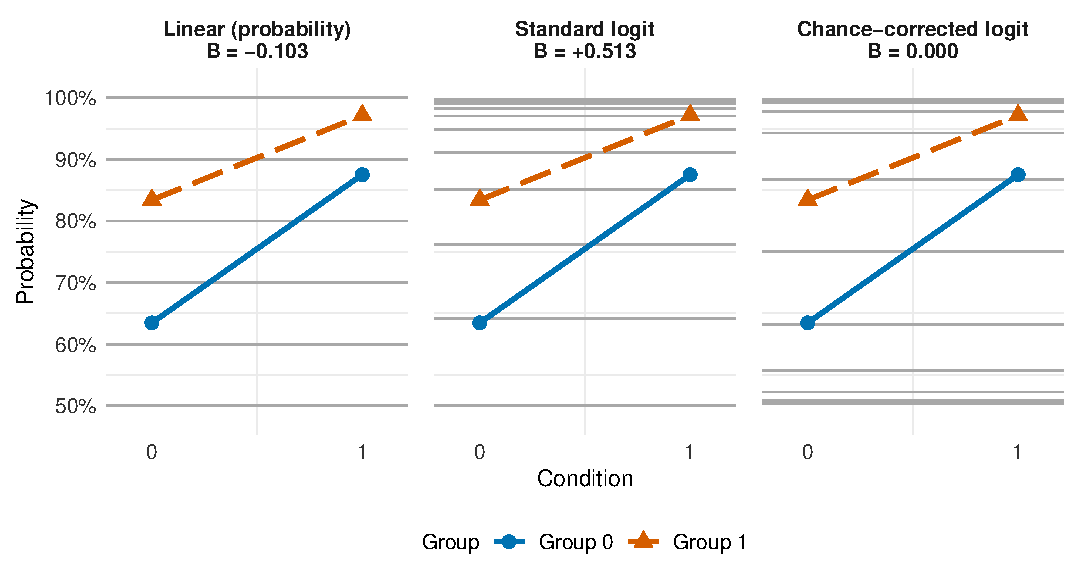
\includegraphics[keepaspectratio]{../figs/motivating-example.pdf}}

}

\end{figure}%

The chance-corrected link is most defensible when the chance level is
known from the task design, guessing is a plausible lower-bound process,
and below-chance performance is not substantively meaningful for the
target claim. In the simplest case, the chance level can be fixed by
design, for example \(c=0.50\) in a two-alternative task. In other
cases, analysts may estimate the lower asymptote or report sensitivity
analyses over plausible values of \(c\). Lapses, response biases, item
heterogeneity, changes across trials, or systematic below-chance
performance may instead require richer psychometric solutions such as
item-response models (e.g., \citeproc{ref-embretsonReise2000}{Embretson
\& Reise, 2000}; \citeproc{ref-knoblauch2012}{Knoblauch \& Maloney,
2012}; \citeproc{ref-wichmann2001}{Wichmann \& Hill, 2001}). For
example, the 3-parameter logistic Item Response Theory model includes an
item-specific guessing parameter rather than a single chance level fixed
at the design level (\citeproc{ref-embretsonReise2000}{Embretson \&
Reise, 2000}). The chance-corrected link should thus be seen as a
design-level approximation, not a substitute for item-level measurement
models when the data and scientific question call for that additional
structure.

\subsubsection{Simulation 1: Design and
Results}\label{simulation-1-design-and-results}

In each of 300 replications we generated accuracy for \(N = 250\)
participants with \(k = 20\) trials each, from a chance-corrected logit
model with a .50 floor, a positive age effect, a group difference, and
no age-by-group product term on the generating scale. Three scenarios
differ only in overall performance, set by shifting the intercept: in
the \emph{lower-performance} scenario the two groups lie close to the
.50 floor (expected accuracies roughly .53 to .80 across ages 6 to 10),
in the \emph{middle-performance} scenario they occupy the middle of the
above-chance range (roughly .55 to .88), and in the
\emph{higher-performance} scenario they approach the ceiling (roughly
.61 to .94). Each simulated dataset was analyzed with four models: a
Gaussian linear model on the observed proportions, standard
binomial-logit and binomial-probit GLMs on the correct-response counts,
and the chance-corrected binomial-logit GLM that matches the generating
scale. We recorded how often each product-term test rejected at
\(\alpha = .05\). The matching model supplies the nominal rejection
rate, while the three alternative scales supply pseudo-interaction
detection rates. Figure~\ref{fig-forced-choice-simulation} shows the
simulation results; the per-scenario rates and the convergence counts
are tabulated in Supplement A.

\begin{figure}[H]

\caption{\label{fig-forced-choice-simulation}Simulation 1: forced-choice
accuracy with a chance floor. Data are generated with no age-by-group
product term on the chance-corrected logit scale. Panel A shows the
resulting accuracy curves across three performance levels; the grey
region lies below the .50 chance floor. Panel B shows product-term
rejection rates by fitted model and scenario. The matched
chance-corrected model remains near nominal alpha, whereas the
alternative scales produce pseudo-interactions. The dashed line marks
alpha = .05.}

\centering{

\pandocbounded{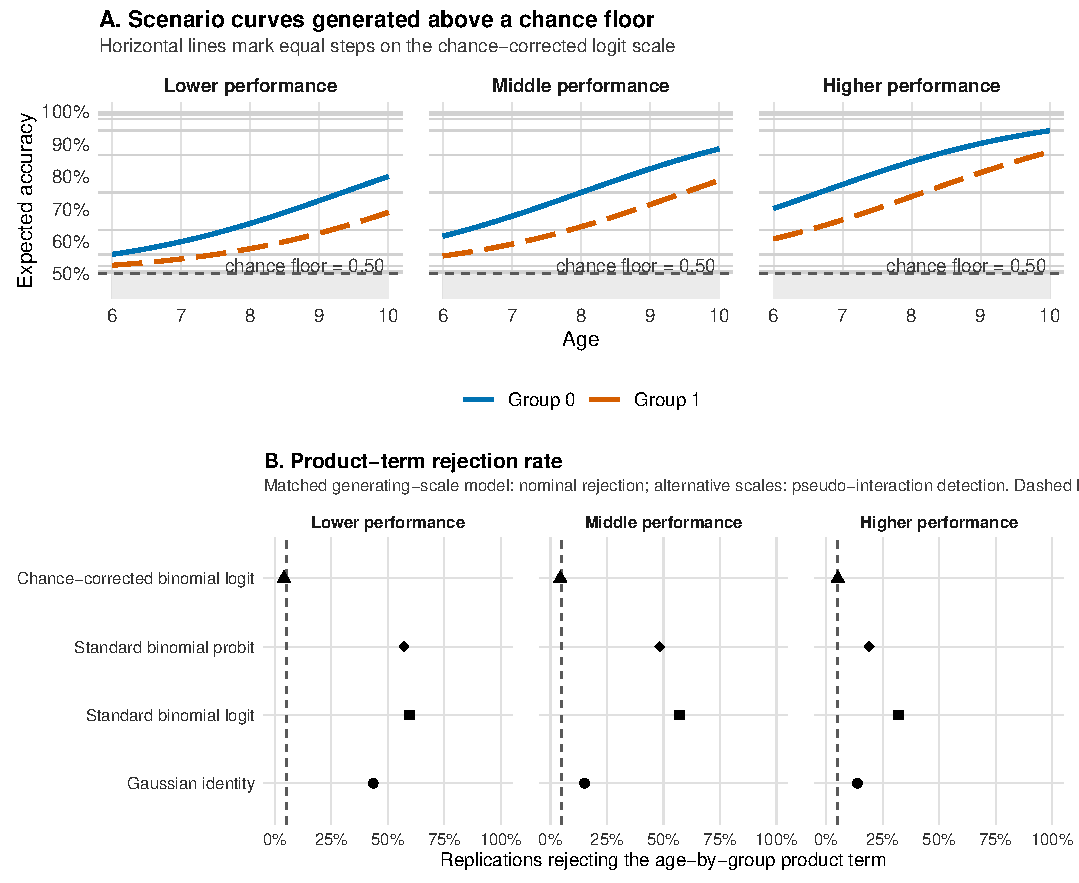
\includegraphics[keepaspectratio]{../figs/forced-choice-simulation.pdf}}

}

\end{figure}%

The chance-corrected model rejects between 2\% and 6\% of the time
across the three scenarios. Pseudo-interaction detection is highest
where performance lies near the floor: in the lower-performance scenario
the standard logit rejects 64\% of the time, the standard probit 61\%,
and the Gaussian identity 46\%. Detection falls as performance moves
away from the floor, reaching 34\% for the logit, 20\% for the probit,
and 12\% for the Gaussian identity in the higher-performance scenario.
The same qualitative sensitivity to the chance floor also appears at
chance levels 0.25 and 0.33 (Supplement B).

Although the chance-corrected model rejects in 2\% of the time in the
lower-performance scenario, the product term there is weakly identified.
As expected accuracy approaches chance, the curve that maps the
above-chance scale onto observed accuracy flattens, so widely different
values on that scale imply almost the same expected accuracies, and the
data cannot distinguish them. Indeed, in the lower-performance scenario
only 164 of the 300 replications produced a usable test of the product
term. The rejection rate is therefore computed on those replications,
and since failures concentrate where the data are least informative
about above-chance differences, they are a selected subset. Restricting
all four models to those 164 replications puts them on identical
datasets and leaves the pattern unchanged. The chance-corrected model
rejects in 2\% of them, against 45\% for the Gaussian identity, 63\% for
the logit, and 62\% for the probit.

\subsection{Within-Family Link Choice}\label{within-family-link-choice}

The forced-choice case involved a link that was plainly wrong for the
task, because it placed the lower asymptote at 0 when the design fixed
it at chance. But the link-function problem can also arise in less
obvious cases. Logit and probit are both standard for binary data,
respect the same 0-to-1 bounds, and usually produce very similar fitted
probabilities. Their choice is therefore often guided by convention,
ease of interpretation, or implementation, with little expected impact
on substantive conclusions (\citeproc{ref-agresti2002}{Agresti, 2002};
\citeproc{ref-yuhuang2019}{Yu \& Huang, 2019}). This makes them a
special case for illustrating the problem, as even two virtually
interchangeable links define slightly different scales of additivity.
Equal differences under one link are not exactly equal under the other,
especially toward the tails, and this alone can alter the estimated
product term.

The logit parameterization also gives coefficients a direct log-odds
interpretation, whereas probit coefficients are expressed on a
standard-normal latent scale, making it a choice of election when
modeling psychological quantities such as ability, signal strength, and
response tendency (\citeproc{ref-dunn2018}{Dunn \& Smyth, 2018}).

\subsubsection{Simulation 2: Design and
Results}\label{simulation-2-design-and-results}

In each of 300 replications we generated repeated binary responses for
\(N = 700\) participants in a two-group, two-condition design, with 15
trials per participant-condition cell and a subject random intercept
(latent intraclass correlation 0.30). The quite large sample was chosen
to make the relatively small systematic discrepancy between logit and
probit links detectable, rather than to represent a typical
psychological study. The condition-by-group interaction term was zero on
the generating link scale. We crossed the generating link with the
fitted link, using logit and probit in both roles, and fitted every
model as a random-intercept GLMM, recording how often each returned a
significant condition-by-group interaction term at \(\alpha = .05\).
Figure~\ref{fig-within-family-links} shows the results; the full
crossed-link rates are tabulated in Supplement A.

\begin{figure}[H]

\caption{\label{fig-within-family-links}Simulation 2: logit versus
probit in repeated-trial random-intercept GLMMs. Data are generated with
no condition-by-group product term on the generating link scale. Panel A
shows the corresponding cell probabilities under logit and probit links.
Panel B shows product-term rejection rates for each generating--fitted
link combination. Matched links remain near nominal alpha, whereas wrong
links produce pseudo-interactions. Error bars are Wilson 95\% confidence
intervals; the dashed line marks alpha = .05.}

\centering{

\pandocbounded{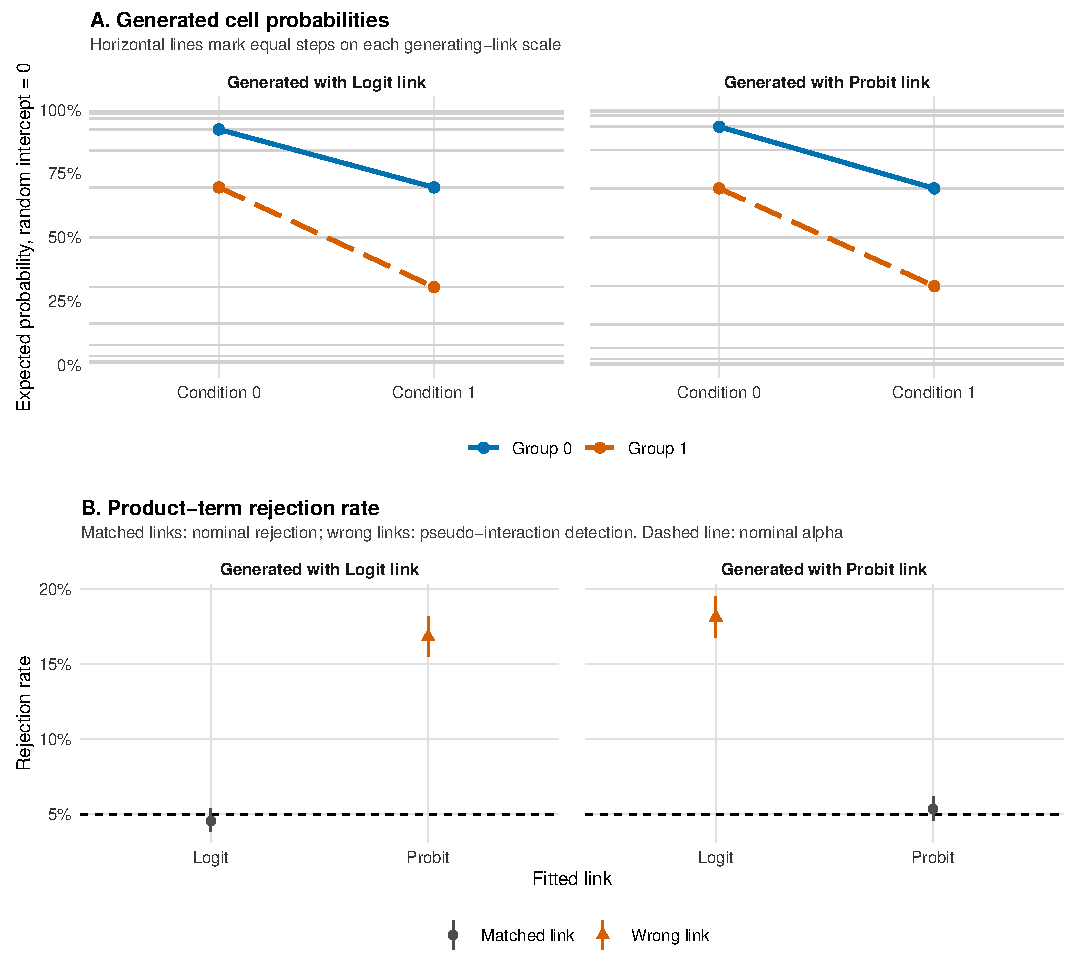
\includegraphics[keepaspectratio]{../figs/within-family-links.pdf}}

}

\end{figure}%

When the fitted link matches the generating link, the nominal rejection
rate stays near .05: 5\% for logit fitted to logit-generated data and
5\% for probit fitted to probit-generated data. Crossing the links
raises the pseudo-interaction detection rate to 14\% when a logit model
is fitted to probit-generated data and 15\% when a probit model is
fitted to logit-generated data, roughly three times the nominal rate.
The wrong-link detection rates are smaller than in the forced-choice
case, and they appear among links that share the same family, the same
0-to-1 bounds, and nearly overlapping fitted curves in the middle of the
probability range, the setting many applied analysts treat as
interchangeable. Under the wrong link the same cell probabilities imply
a small but deterministic nonzero product term on the fitted scale.
Supplement B varies the intercept, which shifts where the four cell
probabilities sit between 0 and 1, and shows that detectability changes
non-monotonically with it, so the same link mismatch is nearly
undetectable at some probability levels and much easier to detect at
others.

A result that is stable across both links is easier to defend; one that
appears only under a single link should be reported as link-conditional.
Supplement A, Section S5, reports how large that fixed product term is.
Taking the cell probabilities implied by each generating model and
re-expressing them on the other link scale gives a product term of
-0.112 for logit-generated data fitted with a probit and 0.216 for
probit-generated data fitted with a logit, against exactly zero whenever
the links match. The rejection rates above are therefore the power to
detect these effects.

\subsection{Sum Scores}\label{sum-scores}

Many psychological outcomes are computed as total sum scores across
questionnaire items, task items, symptoms, errors, or ratings. In the
two cases above the outcome was a directly observed response, and only
the link was in question. A sum score is different, because the score
itself is already the result of an analytic choice. What is observed are
the individual item responses, which are binary or ordinal; the total is
a summary of them, produced by a scoring rule that gives every item the
same weight and every point of the scale the same width. In
psychological research the construct of interest is often the
underlying, generally continuous dimension, so the total can be seen as
a remapped version of that continuum. The link question then arrives
together with a prior question about which metric the claim is about.

The bounds are crucial here, because the construct may have no floor or
ceiling while the observe total score has both. The mapping is best read
as an exchange rate between the two scales, that is, how much of the
latent dimension is needed to gain one raw-score point. That rate is not
constant. Near the middle of the scale a small latent shift is enough to
move the total by a point, while near either bound a wide stretch of the
latent dimension is compressed into the last available point, because
few items remain that the respondent can still change. To illustrate,
with nine items scored 0-3, moving from 13 to 14 points requires less
change on the latent dimension than moving from 26 to 27. A constant
latent effect therefore produces smaller raw-score differences as the
total approaches an end, and the same reasoning applies wherever the
instrument is unevenly informative along the latent dimension, so
compression is not confined to the endpoints.

Bounded, discrete, and skewed distributions are common in psychological
data (\citeproc{ref-micceri1989}{Micceri, 1989}), and the consequences
of analysing ordinal responses as if they were metric have been
documented in detail (\citeproc{ref-liddellkruschke2018}{Liddell \&
Kruschke, 2018}). Fitting a Gaussian identity model to a total assumes
instead that a predictor moves the score by the same number of points at
every level of the other predictor. A group/condition sitting near a
bound moves by fewer points even when the data-generating process on the
latent dimension is the same in both groups/conditions.
Behaviour-genetic research has met the same problem when testing whether
genetic effects vary across environments, since those interactions are
usually tested on summed questionnaire scores: analysed at the item
level, the same data show that the total can conceal real interactions
or present spurious ones through properties of the observed score
(\citeproc{ref-molenaar2014}{Molenaar \& Dolan, 2014}). This is the
sum-score form of outcome-model misspecification and target-metric
mismatch (\citeproc{ref-domingue2024}{Domingue et al., 2024}).

The problem we raise sits next to a recent, wider debate about whether
sum scores should be replaced by factor scores or latent-variable
models. Some argue that sum scores are transparent, reliable enough for
many purposes, comparable across studies, and tied to how instruments
are scored in applied settings (\citeproc{ref-widaman2023}{Widaman \&
Revelle, 2023}); the counterargument is that a total encodes strong and
usually untested assumptions about how items represent the construct
(\citeproc{ref-mcneish2023}{McNeish, 2023};
\citeproc{ref-mcneish2020}{McNeish \& Wolf, 2020}). While we do not
enter the debate, we add a narrower point that was left aside: a model
of the manifest total defines the absence of an interaction in raw-score
points, so an interaction found there is an interaction on the score,
and it becomes a claim about the construct only under the additional
assumption that the two are linearly related.

When item-level data are available and the claim concerns latent
constructs, an explicit measurement model such as SEM, item-level
ordinal regression, or IRT-inspired specifications could be preferred,
since it addresses the mapping directly, though at the price of moving
the assumptions into the measurement model
(\citeproc{ref-burknervuorre2019}{Bürkner \& Vuorre, 2019}). Often,
however, researchers deliberately work with the total score for the
practical reasons listed above. An option is to set a family that
respects the bounds and the discreteness, for example modelling the
total as a bounded count with a beta-binomial likelihood
(\citeproc{ref-wilcox1981}{Wilcox, 1981}). However, we suggest a
deliberately unusual option that moves only the link: keep the observed
total score under a Gaussian likelihood, but rescale the score to the
proportion of the maximum and use a probit link function, as in
Simulation 3 below. This is an \emph{ad hoc} device, not a standard
practice, but it illustrates whether the interaction conclusion changes
if additivity is placed on a nonlinear scale that compresses the
expected values toward the score bounds. It remains a model of the
total, it will not recover the construct, and the Gaussian likelihood is
still misspecified in its variance, since a bounded score has a variance
that depends on its mean: what the probit link corrects is only the
scale on which additivity is defined, not the distributional form. Read
against the sum-score debate, it is a precaution for researchers who
have decided to analyse totals anyway, but acknowledge that the
interaction still needs a scale on which additivity is plausible.

\subsubsection{Simulation 3: Design and
Results}\label{simulation-3-design-and-results}

The bounded-score probit model was compared with two natural
alternatives: the observed total and the latent scale it approximates.
In each of 300 replications, we generated data for \(N = 600\)
participants from a continuous latent variable with a continuous
predictor \(x\), a group effect, and no x-by-group interaction. The
latent values generated 9 ordinal items scored 0 to 3, which were summed
to a total ranging from 0 to 27. Item thresholds were shifted across
three scenarios so that expected totals fell in the middle, lower, or
upper part of the score range.

We analyzed each total in three ways: a Gaussian identity model of the
observed sum score, a Gaussian-probit bounded-score model, and the true
latent generating scale. The bounded-score model applies a probit link
to a continuity-corrected score proportion and rescales predictions to
the original sum-score metric. We used probit because its
standard-normal linear predictor provides a simple correspondence with
the latent scale. This choice is still substantive, as shown in the
previous section. The latent model serves as an idealized benchmark
available only in simulation. We recorded the proportion of significant
x-by-group interactions at \(\alpha = .05\). Results are shown in
Figure~\ref{fig-sum-score-simulation}, with per-scenario rates in
Supplement A, Section S4.

\begin{figure}[H]

\caption{\label{fig-sum-score-simulation}Simulation 3: sum scores as
bounded and discrete outcomes. Data are generated with no x-by-group
product term on the latent scale. Panel A shows how the same additive
latent structure maps onto sum scores in the middle, lower, and upper
parts of the score range. Panel B shows product-term rejection rates for
the latent benchmark and two observed-score models. The latent model
remains near nominal alpha, whereas the observed-score models can
produce pseudo-interactions. The dashed line marks alpha = .05. The
latent benchmark is available only in simulation.}

\centering{

\pandocbounded{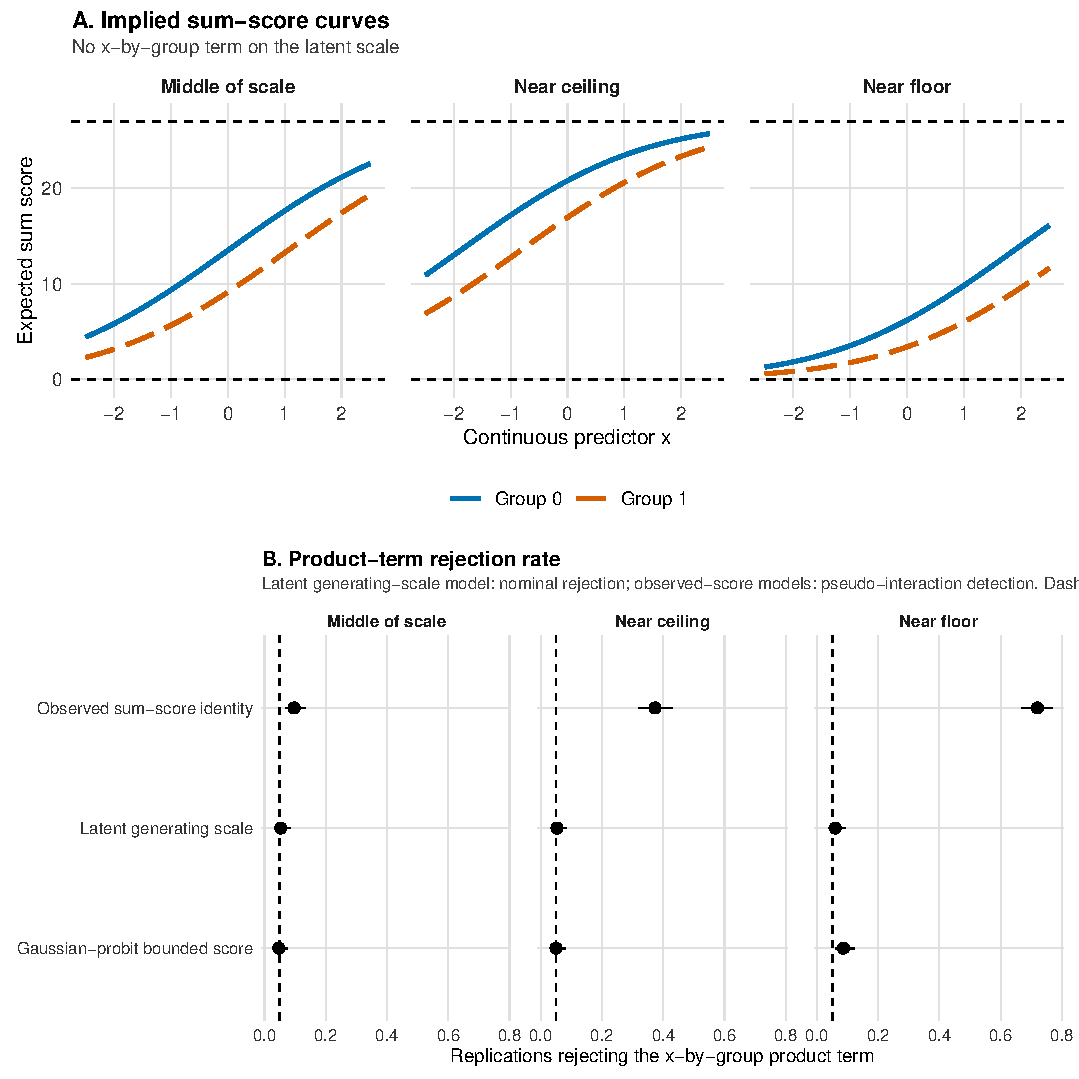
\includegraphics[keepaspectratio]{../figs/sum-score-simulation.pdf}}

}

\end{figure}%

The latent benchmark remained close to the nominal .05 rejection rate in
every scenario, from 5\% to 6\%. The identity model behaved similarly
only in the middle of the score range, where the sum score was
approximately linear in the latent variable (8\%). Rejection increased
as expected totals moved toward a bound, reaching 37\% in the upper
range and 70\% in the lower range. Compression of the latent scale makes
the same latent group difference appear to change across levels of the
predictor. The bounded-score probit model remained close to nominal
alpha across scenarios, from 3\% to 10\%. It respects the score bounds,
although it is still a model of the manifest total.

This pattern mainly depends on where observations fall within the score
range. Across the broader scenarios in Supplement B, the position of
expected scores within the range affected identity-model rejection much
more than sample size, item count, or latent dispersion. Raw-score
additivity can approximate latent-scale additivity when scores remain
away from the bounds. Compression near a bound can instead create an
apparent interaction from a constant latent effect. The bounded-score
probit model can therefore serve as a useful sensitivity analysis. For
claims about interactions between latent constructs, an explicit
measurement model provides a more direct approach, for example SEM,
item-level ordinal models, or IRT-inspired models. These approaches
still depend on assumptions about thresholds, links, loadings, and
latent-response scales, but they make those assumptions part of the
interaction model.

\section{Can Standard Diagnostics Catch a Wrong
Link?}\label{can-standard-diagnostics-catch-a-wrong-link}

The simulations above assume the analyst does not question the fitted
model. In practice, a researcher who finds an interaction may run model
checks before reporting it. We examine the three checks an applied
psychologist is most likely to run, each representing a different
strategy. A Pregibon-style added-term test probes the assumed link,
residual diagnostics screen for misfit of any kind, and AIC ranks a set
of candidate models. Estimating the shape of the link from the data
through a parametric family of links is a more direct strategy, and it
is rarely used in psychology
(\citeproc{ref-aranda-ordaz1981}{Aranda-Ordaz, 1981};
\citeproc{ref-czadosantner1992}{Czado \& Santner, 1992};
\citeproc{ref-stukel1988}{Stukel, 1988}). None of them identifies the
scale on which the no-interaction claim is defined. At best they point
to the link that fits the data best among the alternatives supplied.

A link test of the kind proposed by Pregibon targets link adequacy
directly, in the added-variable form used here
(\citeproc{ref-pregibon1980}{Pregibon, 1980}). The model is fitted, the
fitted linear predictor \(\hat{\eta}\) is extracted, and the model is
refitted with \(\hat{\eta}^2\) added as an extra predictor. If the link
is adequate the squared term carries no additional information and
should be non-significant; a significant term signals curvature that the
current link leaves unexplained. The signal is not specific to the link,
as an omitted nonlinear term, an omitted covariate, or a missing
interaction produce it as well. A non-significant result means only that
this diagnostic did not detect a departure in this sample.

Residual diagnostics start from the position of each observed value
within the distribution the model predicts for that observation. That
position is a number between 0 and 1, and under an adequate model those
positions are uniform whatever the family, which gives residual plots a
common reference distribution and makes misfit visible as departure from
uniformity, as over- or underdispersion, or as residual structure over
fitted values and predictors. Dunn and Smyth pass the position through
the normal quantile function, so their quantile residuals are standard
normal under an adequate model (\citeproc{ref-dunnsmyth1996}{Dunn \&
Smyth, 1996}), while DHARMa obtains the same positions by simulating
datasets from the fitted model and leaves them on the 0-to-1 scale
(\citeproc{ref-hartig2024}{Hartig, 2024}). We use the DHARMa
implementation in R. As with the link test, several causes can produce
departure from uniformity, including link misspecification, wrong
family, missing nonlinearity, missing interaction, and target-metric
mismatch.

Information criteria compare a supplied set of models. We use AIC
throughout, and because our candidate models keeps the response, family,
and structural formula fixed and varies only the link, the ranking
depends entirely on the log-likelihood. Importantly, the result is
restricted to the candidate links that were fitted, and the interaction
term is already present in each model and can absorb part of the
curvature produced by the wrong link. A misspecified model may therefore
fit almost as well as the target model while still placing additivity on
the wrong scale.

\subsection{Diagnostic Simulation}\label{diagnostic-simulation}

The five scenarios reuse examples already introduced in the paper
(Table~\ref{tbl-diagnostic-scenarios}). Each keeps the outcome family
and the interaction formula fixed and changes only the link, so the
fitted model is wrong about the scale on which effects add and about
nothing else. \emph{Count errors} reproduces the Poisson-log example of
Figure~\ref{fig-simple-count-example} and fits it with an identity link.
\emph{Chance-floor accuracy} takes the lower-performance scenario of
Simulation 1, generated on the chance-corrected logit scale and fitted
with a standard binomial logit. \emph{Binary repeated trials} reproduces
the probit-generated, logit-fitted case of Simulation 2. \emph{Binary
continuous predictor} repeats that case with the two-level condition
replaced by a continuous predictor, which allows the residual checks
that need variation along a predictor. \emph{Gamma mean response time}
generates response times from a Gamma model with a log link and fits the
canonical inverse link. The generating parameters for all five are
reported in Supplement A.

In each replication, diagnostics were applied to the misspecified
interaction model, because this is the model an analyst would usually
inspect after obtaining a significant interaction. All rates are
computed over the replications in which that model converged, which is
every one of the 300 replications except in the count scenario, where
the Poisson-identity model returned a usable fit in 281 of them. The
question is therefore whether the same model that produces the
pseudo-interaction also shows enough evidence of misspecification to
warn the analyst.

Each replication was screened with four DHARMa checks, covering residual
uniformity, dispersion, residual quantile patterns over fitted values,
and residual structure over the focal predictor
(\citeproc{ref-dunnsmyth1996}{Dunn \& Smyth, 1996};
\citeproc{ref-hartig2024}{Hartig, 2024}). The last of these takes two
forms, a quantile check when the focal predictor is continuous and a
comparison across design cells in the categorical \(2 \times 2\) case.
Alongside them we ran the Pregibon-style added-term link check
(\citeproc{ref-pregibon1980}{Pregibon, 1980}). Every procedure was
applied a second time to the correctly specified interaction model
fitted to the same data, which calibrates the flagging rates against a
model that is right.

The AIC comparison in each scenario is between the two models already
described, the target and the misspecified one. We report the proportion
of replications in which AIC favored the target model.

\begin{table}

{\caption{{Diagnostic simulation across five link-misspecification
scenarios. Pseudo-interaction reports how often the misspecified model
detected an interaction that was absent on the generating link scale.
DHARMa gives the range across the four prespecified residual checks.
Pregibon reports the added-term link check. AIC favors target reports
the proportion of replications in which the lower AIC favored the target
interaction model over the misspecified interaction model. CI = Wilson
95\% confidence interval. The Pregibon check is not identifiable in the
saturated \(2 \times 2\) design, where the squared linear predictor is
exactly collinear with the existing fixed
effects.}{\label{tbl-diagnostic-scenarios}}}
\vspace{-20pt}}

\begin{longtable}[]{@{}
  >{\raggedright\arraybackslash}p{(\linewidth - 12\tabcolsep) * \real{0.1854}}
  >{\raggedright\arraybackslash}p{(\linewidth - 12\tabcolsep) * \real{0.2119}}
  >{\raggedright\arraybackslash}p{(\linewidth - 12\tabcolsep) * \real{0.1589}}
  >{\raggedleft\arraybackslash}p{(\linewidth - 12\tabcolsep) * \real{0.1589}}
  >{\raggedleft\arraybackslash}p{(\linewidth - 12\tabcolsep) * \real{0.1060}}
  >{\raggedleft\arraybackslash}p{(\linewidth - 12\tabcolsep) * \real{0.0596}}
  >{\raggedleft\arraybackslash}p{(\linewidth - 12\tabcolsep) * \real{0.1192}}@{}}
\toprule\noalign{}
\begin{minipage}[b]{\linewidth}\raggedright
Case
\end{minipage} & \begin{minipage}[b]{\linewidth}\raggedright
Target model
\end{minipage} & \begin{minipage}[b]{\linewidth}\raggedright
Misspecified model
\end{minipage} & \begin{minipage}[b]{\linewidth}\raggedleft
Pseudo-interaction rate
\end{minipage} & \begin{minipage}[b]{\linewidth}\raggedleft
DHARMa
\end{minipage} & \begin{minipage}[b]{\linewidth}\raggedleft
Pregibon
\end{minipage} & \begin{minipage}[b]{\linewidth}\raggedleft
AIC favors target
\end{minipage} \\
\midrule\noalign{}
\endhead
\bottomrule\noalign{}
\endlastfoot
Count errors & Poisson log & Poisson identity & 0.957 {[}0.927, 0.975{]}
& 0.000-0.883 (4) & 0.986 & 0.986 \\
Chance-floor accuracy & chance-corrected binomial logit & standard
binomial logit & 0.587 {[}0.530, 0.641{]} & 0.000-0.060 (4) & 0.317 &
0.813 \\
Binary repeated trials & binomial probit GLMM & binomial logit GLMM &
0.127 {[}0.094, 0.169{]} & 0.000-0.013 (4) & N.A. & 0.950 \\
Binary continuous predictor & binomial probit GLMM & binomial logit GLMM
& 0.073 {[}0.049, 0.109{]} & 0.000-0.003 (4) & 0.043 & 0.937 \\
Gamma mean response time & Gamma log & Gamma inverse & 0.297 {[}0.248,
0.351{]} & 0.000-0.063 (4) & 0.340 & 0.793 \\
\end{longtable}

\end{table}

Table~\ref{tbl-diagnostic-scenarios} shows that the three checks behave
very differently. The Pregibon test flagged the count case in 99\% of
replications, but reached only 34\% in the Gamma case and 32\% at the
chance floor, fell to 4\% for the binary case with a continuous
predictor, and could not be computed at all in the saturated
\(2 \times 2\) design. The DHARMa checks were weaker, reaching 88\% in
the count case and at most 6\% in the other four, so residual screening
responded only where the wrong link visibly distorted the fitted values.
AIC favored the target link in every scenario, from 79\% in the Gamma
case to 99\% in the count case, and was the only check that responded
throughout.

The two logit-probit cases were the hardest to diagnose. They produced
the fewest pseudo-interactions, 13\% in the saturated design and 7\%
with a continuous predictor, and almost nothing detected them, leaving
AIC at 95\% and 94\% as the only informative signal.

The chance-floor scenario is worth a closer look, because it combines a
high pseudo-interaction rate with residual checks that are almost never
significant, which leaves AIC as the only diagnostic that detects the
misspecification. There AIC favored the chance-corrected model in 81\%
of replications, but the margin is often narrow, and Supplement A
reports the full distribution of the AIC difference for every scenario.

Overall, the diagnostics were informative in some settings and weak in
others, even when the pseudo-interaction significance rate is pretty
high. Under the correct link, DHARMa flagged a problem in at most 4.7\%
of replications. Pregibon flagged at most 5.3\% in the count,
chance-floor, and Gamma scenarios, and 4.3\% in the continuous-predictor
GLMM.

Full results are reported in Supplement A, and Supplement B shows how
pseudo-interaction rates, Pregibon detection, and AIC preference change
across sample size and the intercept.

\section{From Link Choice to Sensitivity
Analysis}\label{from-link-choice-to-sensitivity-analysis}

The practical implication of this framework is that an interaction
analysis should make three choices explicit: the link that defines
additivity, the metric the claim refers to, and the sensitivity checks
used to assess that choice (Table~\ref{tbl-link-aware-workflow}). The
observed metric may sometimes be the relevant target. For example, a
two-point difference on a clinical or educational score may be the
quantity that matters in practice, and additivity in raw-score units may
then be reasonable. The key point is that this should be a substantive
choice, not the by-product of using a default model. When possible, the
link should be justified from theory, task structure, or measurement
(\citeproc{ref-baranger2023}{Baranger et al., 2023};
\citeproc{ref-castillo2026}{Castillo et al., 2026}).

When link choice can affect the interaction conclusion, we suggest that
the main robustness check is to performa a sensitivity analysis across
plausible links. Researchers should therefore compare the same target
response-scale contrast across alternatives and report whether the
result is stable or link-conditional. If it changes, that dependence is
itself part of the result (\citeproc{ref-mccabe2022}{McCabe et al.,
2022}; \citeproc{ref-mize2019}{Mize, 2019};
\citeproc{ref-mustillo2018}{Mustillo et al., 2018};
\citeproc{ref-rohrer2026}{Rohrer \& Arel-Bundock, 2026}).

\begin{table}

{\caption{{Practical starting points for link-aware interaction testing
across common psychological outcomes.}{\label{tbl-link-aware-workflow}}}
\vspace{-20pt}}

\begin{longtable}[]{@{}
  >{\raggedright\arraybackslash}p{(\linewidth - 4\tabcolsep) * \real{0.2000}}
  >{\raggedright\arraybackslash}p{(\linewidth - 4\tabcolsep) * \real{0.4200}}
  >{\raggedright\arraybackslash}p{(\linewidth - 4\tabcolsep) * \real{0.3800}}@{}}
\toprule\noalign{}
\begin{minipage}[b]{\linewidth}\raggedright
Outcome type
\end{minipage} & \begin{minipage}[b]{\linewidth}\raggedright
Plausible starting point
\end{minipage} & \begin{minipage}[b]{\linewidth}\raggedright
Minimal sensitivity check
\end{minipage} \\
\midrule\noalign{}
\endhead
\bottomrule\noalign{}
\endlastfoot
Forced-choice accuracy & Binomial logit/probit; chance-corrected link
when the task floor is part of the estimand. & Compare standard
logit/probit and chance-corrected links; report convergence and
response-scale contrasts. \\
Binary / proportion outcome & Binomial logit/probit; consider cloglog
for asymmetric processes. & Compare logit/probit; inspect calibration
and contrasts near bounds or rare-event regions. \\
Likert / ordinal item & Ordinal logit/probit; metric model only with a
clear observed-scale target. & Compare ordinal and metric summaries;
report category probabilities or response-scale contrasts. \\
Sum score / composite & Gaussian identity when many levels stay far from
bounds; otherwise consider item-level, ordinal, bounded-count, or
bounded-score models. & Inspect bounds, skew, and score concentration;
compare with item-level or bounded-score sensitivity models when
feasible. \\
Counts / error counts & Poisson or negative binomial, usually with log
link; identity only with an observed-count target. & Check
overdispersion and zero inflation; compare count contrasts across
plausible count models. \\
Response time / skewed positive outcome & Lognormal, Gamma log/inverse,
Inverse Gaussian, or transformed Gaussian, matched to absolute,
proportional, reciprocal, or transformed change. & Compare raw-, log-,
and response-scale summaries; inspect tail fit and predicted values. \\
\end{longtable}

\end{table}

\section{Discussion}\label{discussion}

The same data can support different interaction conclusions under
different plausible specifications, which is the familiar scale
dependence of interactions (\citeproc{ref-cox1984}{Cox, 1984};
\citeproc{ref-loftus1978}{Loftus, 1978};
\citeproc{ref-wagenmakers2012}{Wagenmakers et al., 2012}). In a GLM that
dependence is carried by two choices, the outcome family and the link
function. Our review found interaction tests to be common in all five
journals sampled, the link function usually left implicit, and
identity-link analyses applied to many outcomes for which observed-scale
additivity is not self-evident.

The simulations then showed what that can cost. With two main effects
present, a link that misplaces additivity turned a purely additive
generating process into a significant product term even when the outcome
family was correct. In forced-choice accuracy the binomial family is
correct and the error lies entirely in a canonical link that places the
lower asymptote at 0 rather than at the chance level. The logit-probit
comparison showed that the problem survives when the response bounds are
correct as well, between two links that look alike over most of the
range. In the sum-score case the choice extends beyond the link to the
outcome itself. A total is a scoring rule applied to item responses, so
an interaction estimated on it refers to raw-score points, and adopting
a family that respects the bounds and the discreteness of the total
still leaves open whether additivity in points stands for additivity in
the construct.

This difficulty is of a different kind from the one documented in work
on the precision of interaction estimates
(\citeproc{ref-baranger2023}{Baranger et al., 2023};
\citeproc{ref-castillo2026}{Castillo et al., 2026}). There the obstacle
is noise, and more data helps. Here the product term induced by the
wrong link is a fixed property of that scale, so a larger sample
estimates it more precisely and reports it as significant more often.

The diagnostic simulation showed that ordinary post-fit checks catch
this unevenly. Residual checks, Pregibon-style tests, and AIC each
detected the misspecification in some scenarios and not in others, and
their sensitivity depended on which candidate models were supplied. The
chance-floor scenario illustrates this most clearly, since a wrong link
produced pseudo-interactions in most replications while the residual
checks were almost never significant, and the only check that detected
the misspecification was the explicit comparison between the two
candidate links, which preferred the correct link by a narrow margin.
These diagnostics therefore answer a question about fit within a
supplied candidate set, which is a different question from whether an
interaction claim holds on the scale the researcher means
(\citeproc{ref-dunnsmyth1996}{Dunn \& Smyth, 1996};
\citeproc{ref-hartig2024}{Hartig, 2024};
\citeproc{ref-pregibon1980}{Pregibon, 1980}).

Three limitations bound the scope of these conclusions. The review was
descriptive and covered five reference journals across major areas of
psychology in a single year, so its estimates describe reporting
practice in high-standard outlets rather than the field as a whole, and
a broader mapping across journals, years, and subfields would be needed
to support reporting guidance. The review also coded observable
reporting features and did not judge, article by article, whether a
given interaction was scale-dependent enough to be removable. The
simulations, finally, are demonstrations of a mechanism. They target a
single regime, in which two established main effects push expected
values into the region where link curvature is strongest, and they say
nothing about how often that regime arises or about the further
complications of real data.

To conclude, interaction claims rest on a scale that is rarely stated.
Naming it separates three questions that a software default otherwise
settles at once, which family suits the response, which link defines
additivity, and which metric the claim is about. The robustness question
then takes a definite form, whether the conclusion survives the links
that remain defensible. A result that holds across them is robust to
that choice. One that does not is still a result, and it should be
reported as conditional on the scale on which it was estimated.

\section{References}\label{references}

\phantomsection\label{refs}
\begin{CSLReferences}{1}{0}
\bibitem[\citeproctext]{ref-agresti2002}
Agresti, A. (2002). \emph{Categorical data analysis} (2nd ed.). John
Wiley \& Sons.

\bibitem[\citeproctext]{ref-ainorton2003}
Ai, C., \& Norton, E. C. (2003). Interaction terms in logit and probit
models. \emph{Economics Letters}, \emph{80}(1), 123--129.
\url{https://doi.org/10.1016/S0165-1765(03)00032-6}

\bibitem[\citeproctext]{ref-aranda-ordaz1981}
Aranda-Ordaz, F. J. (1981). On two families of transformations to
additivity for binary response data. \emph{Biometrika}, \emph{68}(2),
357--363. \url{https://doi.org/10.1093/biomet/68.2.357}

\bibitem[\citeproctext]{ref-baranger2023}
Baranger, D. A. A., Finsaas, M. C., Goldstein, B. L., Vize, C. E.,
Lynam, D. R., \& Olino, T. M. (2023). Tutorial: Power analyses for
interaction effects in cross-sectional regressions. \emph{Advances in
Methods and Practices in Psychological Science}, \emph{6}(3),
10.1177/25152459231187531.
\url{https://doi.org/10.1177/25152459231187531}

\bibitem[\citeproctext]{ref-burknervuorre2019}
Bürkner, P.-C., \& Vuorre, M. (2019). Ordinal regression models in
psychology: A tutorial. \emph{Advances in Methods and Practices in
Psychological Science}, \emph{2}(1), 77--101.
\url{https://doi.org/10.1177/2515245918823199}

\bibitem[\citeproctext]{ref-busemeyer1983}
Busemeyer, J. R., \& Jones, L. E. (1983). Analysis of multiplicative
combination rules when the causal variables are measured with error.
\emph{Psychological Bulletin}, \emph{93}(3), 549--562.
\url{https://doi.org/10.1037/0033-2909.93.3.549}

\bibitem[\citeproctext]{ref-castillo2026}
Castillo, A., Miller, J. D., Vize, C., Baranger, D. A. A., \& Lynam, D.
R. (2026). When do interaction/moderation effects stabilize in linear
regression? \emph{Advances in Methods and Practices in Psychological
Science}, \emph{9}(1), 10.1177/25152459251407860.
\url{https://doi.org/10.1177/25152459251407860}

\bibitem[\citeproctext]{ref-cox1984}
Cox, D. R. (1984). Interaction. \emph{International Statistical Review /
Revue Internationale de Statistique}, \emph{52}(1), 1--24.
\url{https://doi.org/10.2307/1403235}

\bibitem[\citeproctext]{ref-czadosantner1992}
Czado, C., \& Santner, T. J. (1992). The effect of link misspecification
on binary regression inference. \emph{Journal of Statistical Planning
and Inference}, \emph{33}(2), 213--231.
\url{https://doi.org/10.1016/0378-3758(92)90069-5}

\bibitem[\citeproctext]{ref-domingue2024}
Domingue, B. W., Kanopka, K., Trejo, S., Rhemtulla, M., \& Tucker-Drob,
E. M. (2024). Ubiquitous bias and false discovery due to model
misspecification in analysis of statistical interactions: The role of
the outcome{'}s distribution and metric properties. \emph{Psychological
Methods}, \emph{29}(6), 1164--1179.
\url{https://doi.org/10.1037/met0000532}

\bibitem[\citeproctext]{ref-dunnsmyth1996}
Dunn, P. K., \& Smyth, G. K. (1996). Randomized quantile residuals.
\emph{Journal of Computational and Graphical Statistics}, \emph{5}(3),
236--244. \url{https://doi.org/10.1080/10618600.1996.10474708}

\bibitem[\citeproctext]{ref-dunn2018}
Dunn, P. K., \& Smyth, G. K. (2018). \emph{Generalized {Linear Models
With Examples} in {R}}. Springer New York.
\url{https://doi.org/10.1007/978-1-4419-0118-7}

\bibitem[\citeproctext]{ref-embretsonReise2000}
Embretson, S. E., \& Reise, S. P. (2000). \emph{Item response theory for
psychologists}. Lawrence Erlbaum Associates.
\url{https://doi.org/10.4324/9781410605269}

\bibitem[\citeproctext]{ref-hartig2024}
Hartig, F. (2024). \emph{{DHARMa}: Residual diagnostics for hierarchical
(multi-level / mixed) regression models}.
\url{https://doi.org/10.32614/CRAN.package.DHARMa}

\bibitem[\citeproctext]{ref-knoblauch2012}
Knoblauch, K., \& Maloney, L. T. (2012). \emph{Modeling Psychophysical
Data in R}. Springer. \url{https://doi.org/10.1007/978-1-4614-4475-6}

\bibitem[\citeproctext]{ref-liddellkruschke2018}
Liddell, T. M., \& Kruschke, J. K. (2018). Analyzing ordinal data with
metric models: What could possibly go wrong? \emph{Journal of
Experimental Social Psychology}, \emph{79}, 328--348.
\url{https://doi.org/10.1016/j.jesp.2018.08.009}

\bibitem[\citeproctext]{ref-loftus1978}
Loftus, G. R. (1978). On interpretation of interactions. \emph{Memory \&
Cognition}, \emph{6}(3), 312--319.
\url{https://doi.org/10.3758/BF03197461}

\bibitem[\citeproctext]{ref-lubinski1990}
Lubinski, D., \& Humphreys, L. G. (1990). Assessing spurious
{"}moderator effects{"}: Illustrated substantively with the hypothesized
({"}synergistic{"}) relation between spatial and mathematical ability.
\emph{Psychological Bulletin}, \emph{107}(3), 385--393.
\url{https://doi.org/10.1037/0033-2909.107.3.385}

\bibitem[\citeproctext]{ref-mccabe2022}
McCabe, C. J., Halvorson, M. A., King, K. M., Cao, X., \& Kim, D. S.
(2022). Interpreting interaction effects in generalized linear models of
nonlinear probabilities and counts. \emph{Multivariate Behavioral
Research}, \emph{57}(2-3), 243--263.
\url{https://doi.org/10.1080/00273171.2020.1868966}

\bibitem[\citeproctext]{ref-mccullaghnelder1989}
McCullagh, P., \& Nelder, J. A. (1989). \emph{Generalized linear models}
(2nd ed.). Chapman; Hall.

\bibitem[\citeproctext]{ref-mcneish2023}
McNeish, D. (2023). Psychometric properties of sum scores and factor
scores differ even when their correlation is 0.98: A response to Widaman
and Revelle. \emph{Behavior Research Methods}, \emph{55}(8), 4269--4290.
\url{https://doi.org/10.3758/s13428-022-02016-x}

\bibitem[\citeproctext]{ref-mcneish2020}
McNeish, D., \& Wolf, M. G. (2020). Thinking twice about sum scores.
\emph{Behavior Research Methods}, \emph{52}(6), 2287--2305.
\url{https://doi.org/10.3758/s13428-020-01398-0}

\bibitem[\citeproctext]{ref-micceri1989}
Micceri, T. (1989). The unicorn, the normal curve, and other improbable
creatures. \emph{Psychological Bulletin}, \emph{105}(1), 156--166.

\bibitem[\citeproctext]{ref-mize2019}
Mize, T. D. (2019). Best practices for estimating, interpreting, and
presenting nonlinear interaction effects. \emph{Sociological Science},
\emph{6}, 81--117. \url{https://doi.org/10.15195/v6.a4}

\bibitem[\citeproctext]{ref-molenaar2014}
Molenaar, D., \& Dolan, C. V. (2014). Testing systematic genotype by
environment interactions using item level data. \emph{Behavior
Genetics}, \emph{44}(3), 212--231.
\url{https://doi.org/10.1007/s10519-014-9647-9}

\bibitem[\citeproctext]{ref-mustillo2018}
Mustillo, S. A., Lizardo, O. A., \& McVeigh, R. M. (2018). Editors{'}
Comment: A Few Guidelines for Quantitative Submissions. \emph{American
Sociological Review}, \emph{83}(6), 1281--1283.
\url{https://doi.org/10.1177/0003122418806282}

\bibitem[\citeproctext]{ref-nelderwedderburn1972}
Nelder, J. A., \& Wedderburn, R. W. M. (1972). Generalized linear
models. \emph{Journal of the Royal Statistical Society: Series A
(General)}, \emph{135}(3), 370--384.
\url{https://doi.org/10.2307/2344614}

\bibitem[\citeproctext]{ref-pregibon1980}
Pregibon, D. (1980). Goodness of link tests for generalized linear
models. \emph{Journal of the Royal Statistical Society Series C: Applied
Statistics}, \emph{29}(1), 15--24. \url{https://doi.org/10.2307/2346405}

\bibitem[\citeproctext]{ref-rimpler2026}
Rimpler, A., Kiers, H. A. L., \& Ravenzwaaij, D. van. (2026). Anything
Goes: Statistical Interactions Without Substantive Theory.
\emph{Computational Brain \& Behavior}.
\url{https://doi.org/10.1007/s42113-026-00305-8}

\bibitem[\citeproctext]{ref-rohrer2026}
Rohrer, J. M., \& Arel-Bundock, V. (2026). Models as Prediction
Machines: How to Convert Confusing Coefficients Into Clear Quantities.
\emph{Advances in Methods and Practices in Psychological Science},
\emph{9}(2), 25152459261424825.
\url{https://doi.org/10.1177/25152459261424825}

\bibitem[\citeproctext]{ref-rohrer2021}
Rohrer, J. M., \& Arslan, R. C. (2021). Precise Answers to Vague
Questions: Issues With Interactions. \emph{Advances in Methods and
Practices in Psychological Science}, \emph{4}(2), 25152459211007368.
\url{https://doi.org/10.1177/25152459211007368}

\bibitem[\citeproctext]{ref-stukel1988}
Stukel, T. A. (1988). Generalized logistic models. \emph{Journal of the
American Statistical Association}, \emph{83}(402), 426--431.
\url{https://doi.org/10.1080/01621459.1988.10478613}

\bibitem[\citeproctext]{ref-wagenmakers2012}
Wagenmakers, E.-J., Krypotos, A.-M., Criss, A. H., \& Iverson, G.
(2012). On the interpretation of removable interactions: A survey of the
field 33~years after Loftus. \emph{Memory \& Cognition}, \emph{40}(2),
145--160. \url{https://doi.org/10.3758/s13421-011-0158-0}

\bibitem[\citeproctext]{ref-wichmann2001}
Wichmann, F. A., \& Hill, N. J. (2001). The psychometric function: I.
Fitting, sampling, and goodness of fit. \emph{Perception \&
Psychophysics}, \emph{63}(8), 1293--1313.
\url{https://doi.org/10.3758/BF03194544}

\bibitem[\citeproctext]{ref-widaman2023}
Widaman, K. F., \& Revelle, W. (2023). Thinking thrice about sum scores,
and then some more about measurement and analysis. \emph{Behavior
Research Methods}, \emph{55}(2), 788--806.
\url{https://doi.org/10.3758/s13428-022-01849-w}

\bibitem[\citeproctext]{ref-wilcox1981}
Wilcox, R. R. (1981). A review of the beta-binomial model and its
extensions. \emph{Journal of Educational Statistics}, \emph{6}(1),
3--32. \url{https://doi.org/10.2307/1165046}

\bibitem[\citeproctext]{ref-yuhuang2019}
Yu, S., \& Huang, X. (2019). Link misspecification in generalized linear
mixed models with a random intercept for binary responses. \emph{TEST},
\emph{28}(3), 827--843. \url{https://doi.org/10.1007/s11749-018-0602-6}

\end{CSLReferences}






\end{document}
